\documentclass[a4paper]{article}
\usepackage[warn]{mathtext}
\usepackage[utf8]{inputenc}
\usepackage[T2A]{fontenc}

\usepackage[english,russian]{babel}
\usepackage{multicol}
\usepackage{fancyhdr}
\usepackage{graphicx}
\usepackage{microtype}
\usepackage{wrapfig}
\usepackage{amsmath}
\usepackage{floatflt}
\usepackage{geometry} \geometry{verbose,a4paper,tmargin=2cm,bmargin=2cm,lmargin=1.5cm,rmargin=1.5cm}
\usepackage{float}
\usepackage{amssymb}
\usepackage{caption}
\usepackage{epsfig}
\usepackage{newunicodechar}

\begin{document}

\graphicspath{ {pictures/} }

\begin{titlepage}
	\centering
	\vspace{5cm}
    {\scshape\LARGE Московский физико-технический институт\par}
	\vspace{5cm}
	{\scshape\Large Лабораторная работа по общей физике \par}
	\vspace{1cm}
    {\huge\bfseries  №4.4.1 Амлитудная дифракционая решетка   \par}
	\vspace{1cm}
	\vfill
    \begin{flushright}
        {\large выполнил студент Б01-903 группы ФРКТ}\par
        \vspace{0.3cm}
        {\LARGE Прохорова Юлия}
    \end{flushright}
	\vfill
Долгопрудный, 2021
% Bottom of the page
\end{titlepage}

\pagestyle{fancy} 
\fancyhead[L]{Оптика}
\fancyhead[R]{Амплитудная диффракционная решетка}
\fancyfoot[C]{ \noindent\rule{\textwidth}{0.4pt} \thepage }

\tableofcontents

\newpage



\section{Цель работы}

Занкомство с работой и настройка гониометра Г5, определение спектральных характеристик амлитудной решетки.

\section{Оборудование}

\begin{itemize}
    \item Гониометр 
    \item Амлитудная дифракционная решетка 
    \item Ртутная лампа 
    \item Призменный уголговый отражатель
    \item Щель с микрометрическим винтом
\end{itemize}

\section{Теория}

\subsection{Общие понятия}
Оптические приборы, в которых осуществялется физическое разложение электромагнитного излучения намонозроматические составляющие, называютсяспектральными. По характеру распределения интенсивности вспектральном разложении спектры могут быть ращделены налинейчатыеинепрерывные. \par 
Принципиальная установка изображена на рис.\ref{p1}. Свет от источника S попадает на экран с щелью. Колли-матор формирует близкие к параллельному пучок лучей. После, свет попадает надиспергирующий элемент.Наблюдейние производится через трубу, установленну на $\infty$


\begin{figure}[H]
    \begin{center}
        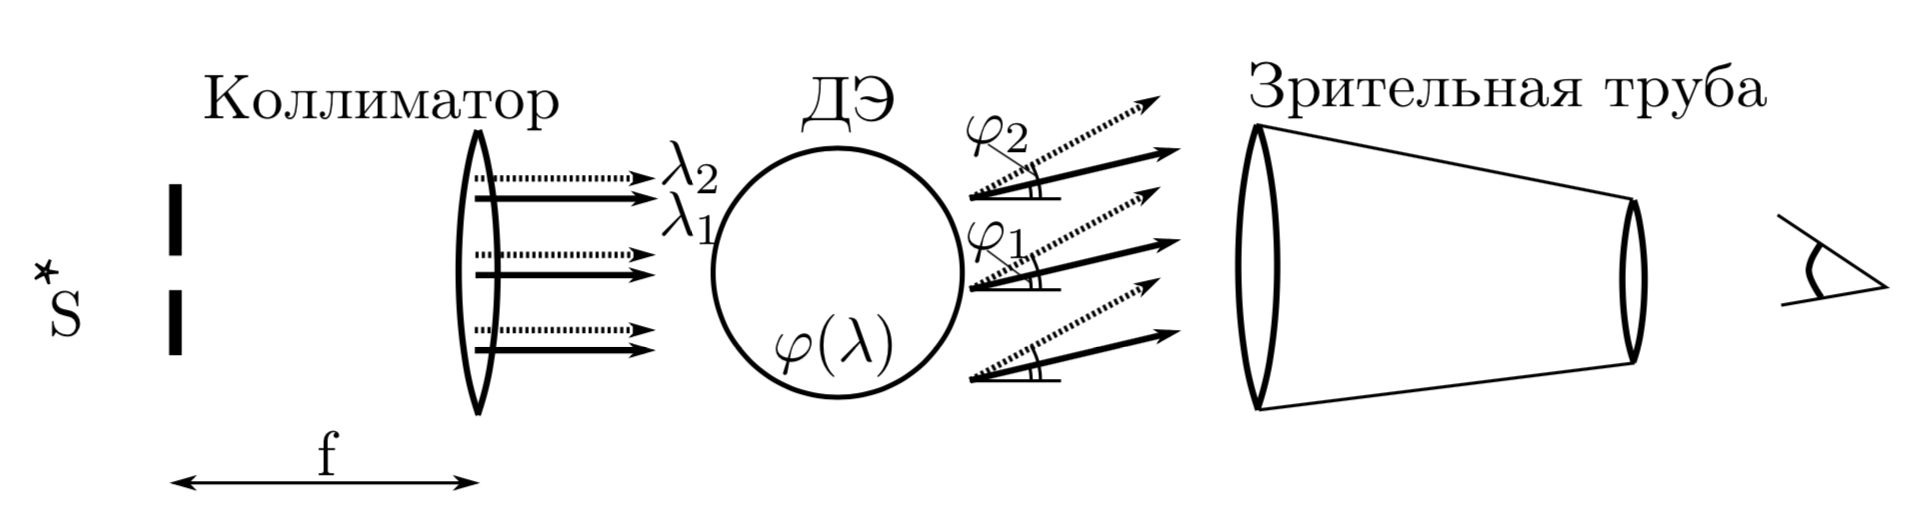
\includegraphics[scale = 0.5]{p1.png}
        \caption{Схема прибора: источник-коллиматор – диспергирующий элемент – зрительная труба}
        \label{p1}
    \end{center}
\end{figure}

Каждой монохроматической компоненте с $\lambda$ соответствует один или несколько углов $\varphi(\lambda)$ на выходе изприбора, в направлении которых интенсивность прибора максимальна. При известной зависимости $\varphi(\lambda)$ поизмеряемому углу поворота $\varphi$ зрительной трубы можно определить длинну волны спектральной линии. \par 
Наиболее важными характеристиками спектральных приборов являютсяугловая дисперсия, разрешающая способность и дисперсионная область.


\subsection{Амплитудная дифракционная решетка}

Амплитадная решетка представляет собой N паралельных щелей (рис.2), период решетки равен d, ширинаштриха - b. Наблюдение ведем на бесконечности (дифракция Фраунгофера). Амплитуда и интенсивность поля
световой волны определяются углом $\varphi$. Полагаем, что амплитуда падающих лучей одинкова. Интенсивность дифрагированного света максимальная для углов $\varphi_m$, при которых волны, приходящие в точку наблюдения оказываются в фазе:

\begin{equation}
    d \sin{\varphi_m} m\lambda
\end{equation}

\begin{figure}[H]
    \begin{center}
    \begin{minipage}[h]{0.3\linewidth}
    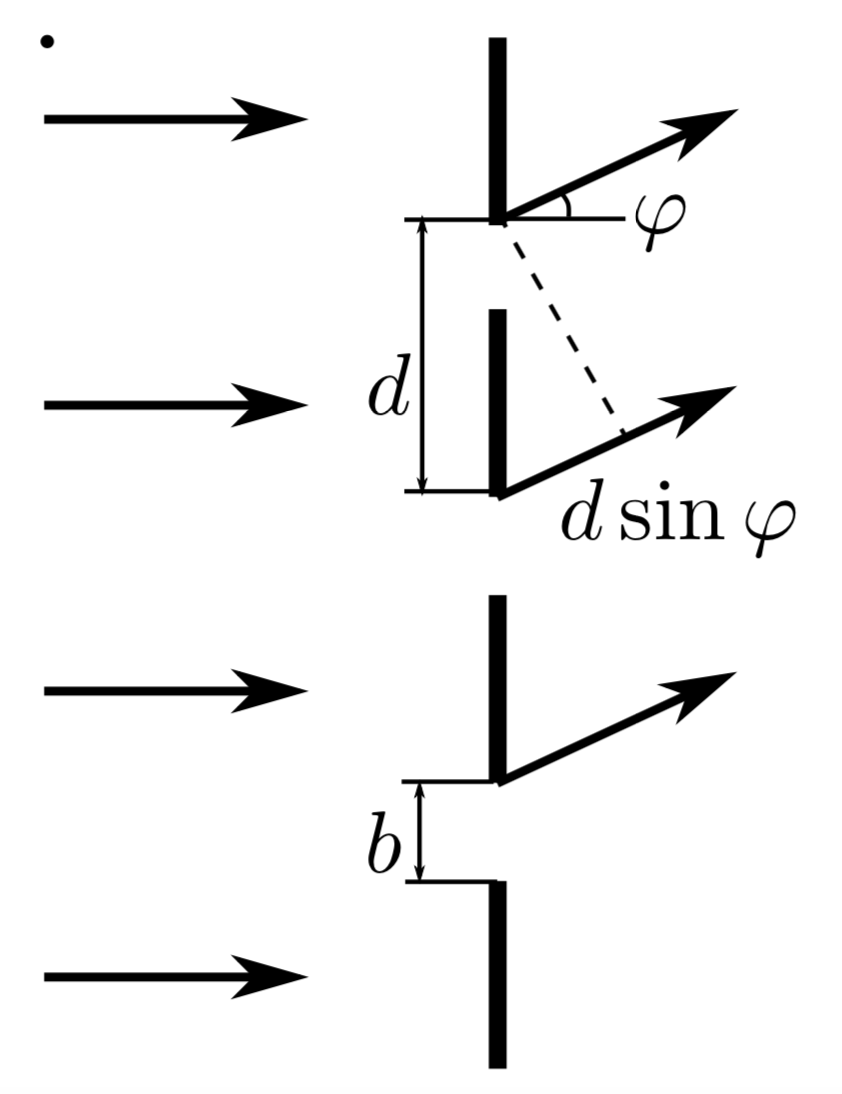
\includegraphics[width=1\linewidth]{p2.png}
    \caption{Дифракция световой волны на амплитудной решетке} 
    \label{p2}
    \end{minipage}
    \hfill 
    \begin{minipage}[h]{0.45\linewidth}
    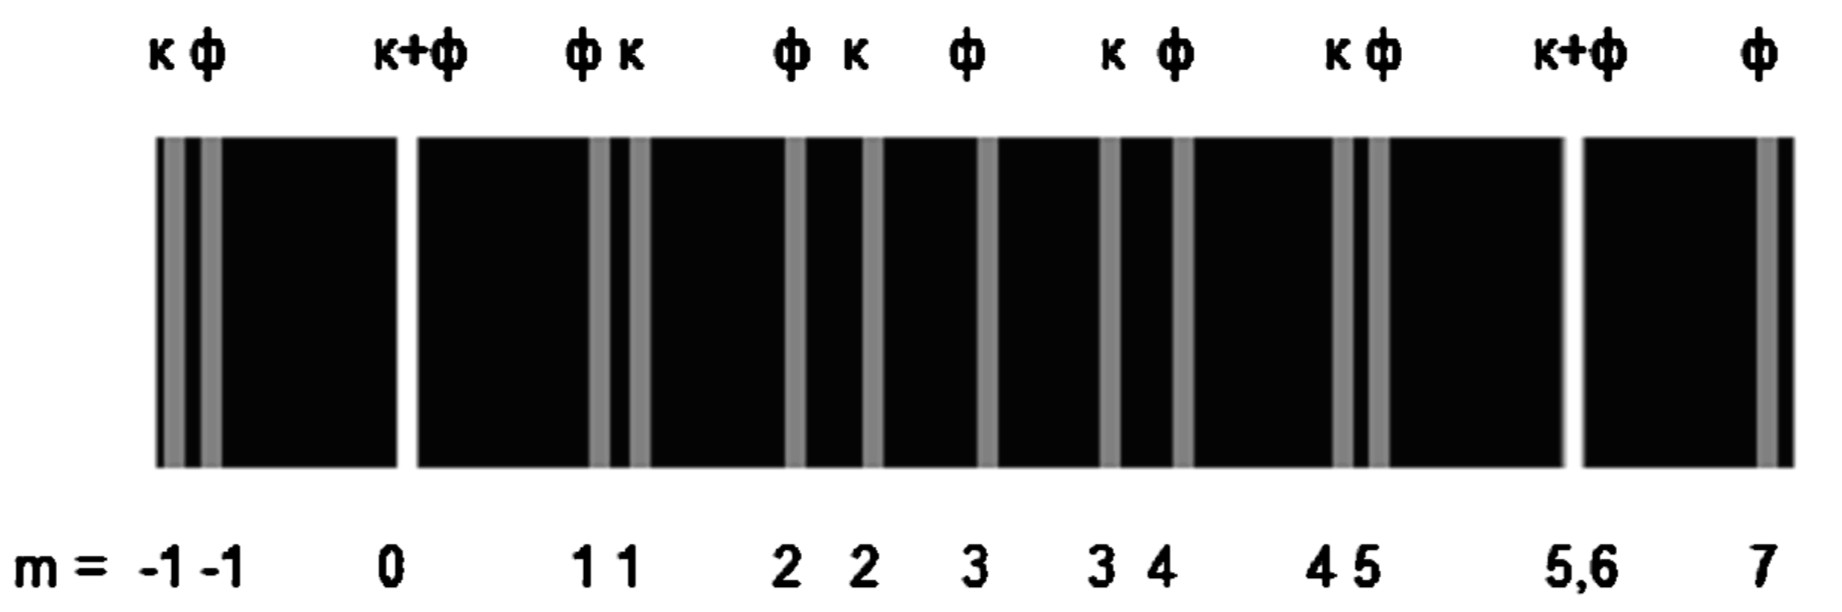
\includegraphics[width=1\linewidth]{p3.png}
    \caption{Изображение спектра двух линий}
    \label{p3}
    \end{minipage}
    \end{center}
\end{figure}

Рассмотрим пример с двумя спектральными линиями красной и фиолетовой $(\lambda_{red}> \lambda_{purp})$ рис.3. Для малых углов дифракции угловое расстояние между порядками $\varphi_{m+1} - \varphi \approx \lambda /d$ пропорционально длине волны, поэтому фиолетовые линии следуют чаще чем красные. При m = 5 для красной и m = 6 для фиолетовой они совпадут. \par 

Некоторые формулы:

\begin{itemize}
    \item Разрешающая способность характеризует возможность прибора различать две близкие спектральные линии с длинами волн $\lambda$ и $\lambda + \delta \lambda$.
    \begin{equation}
        R = \frac{\lambda}{\delta \lambda}
    \end{equation}

    \item Угловая дисперсия - производная зависимости угла отклонения $\varphi(\lambda)$ волны диспергирующим элементом по $\lambda$. По величине угловой дисперсии можно определить угловое расстояние между двумя близкими спектральными линиями: $\delta \varphi \approx D \delta \lambda$:

    \begin{equation}
        D = \frac{d \varphi}{d \lambda} = \frac{m}{d \cdot \cos{\varphi_m}} = \frac{m}{\sqrt{d^2 - m^2 \lambda^2}}
    \end{equation}

    \item Угловое расстояние между линиями определяется:
    \begin{equation}
        \Delta \varphi \approx D \delta \lambda
    \end{equation}

    \item Поулширина линии:
    \begin{equation}
        \delta \varphi = \frac{\lambda}{Nd \cos{\varphi_m}}
    \end{equation}

    \item Дисперсионная область – предельная ширина спектального интервала $\Delta \lambda$ прибора, для которой дифракционные максимумы соседних порядков не перекрываются. Она определяет диапазон длин волн, при которых прибор может быть использован для анализа спектра.

\end{itemize}


\section{Ход работы}

\begin{enumerate}
    \item Настроим гониометр
    \item Установили решетку, откалиьбровали наклон столика.
    \item Подберем ширину входной щели так, чтобы ширина желктого дуплета была чуть больше промежуткамежду линиями двойного штриха окуляра.
    \item Измерим угловые координаты спектральных линий ртути в±1порядке и занесем в таблицу \ref{t1}

    \begin{table}[H]
        \begin{center}
            \begin{tabular}{|c|c|c|c|}
                \hline
                Цвет & Угол & Длина волны, $\lambda, \; нм$ & Порядок \\ \hline 
                Фиолетовый & 192 $^{\circ}$ 33'&404.66& 1\\ \hline
                Зеленый & 194 $^{\circ}$ 10' & 546.07 & 1 \\\hline
                Желтый & 196 $^{\circ}$ 41' &576.96 & 1 \\ \hline
                Красный & 197 $^{\circ}$ 35' & 690.72 & 1\\ \hline
                Фиолетовый & 167 $^{\circ}$ 24' & 404.66 & -1 \\ \hline 
                Зеленый & 164 $^{\circ}$ 09' & 546.07 & -1 \\\hline
                Желтый & 163 $^{\circ}$ 12' &576.96 & -1 \\ \hline
                Красный & 161 $^{\circ}$ 50' & 690.72 & -1\\ \hline
                
            \end{tabular}
            \caption{}
            \label{t1}
        \end{center}
    \end{table}

    \item Построим зависимость $\sin{\varphi_m}$ от длины волны:
    \item По формуле $d \sin{\varphi_m} = m \lambda$ и наклону графика определим период решетки:
    $$d = \frac{\delta \lambda}{\delta \varphi} = $$

    \item Для оценки угловой дисперсии решетки измерим угловые координаты линий желтого дуплета на всехвидимых порядках, результат занесем в таблицу \ref{t2}.
    
    \begin{table}[H]
        \begin{center}
            \begin{tabular}{|c|c|c|c|c|c|c|c|c|}
                \hline
                Порядок&-1&-1&1&1&2&2&-2&-2 \\ \hline 
                $\lambda, \;nm$&576.96&579.09&576.96&579.07&579.96&576.09&576.96&579.07 \\ \hline
                $\Delta \lambda, \; nm$& -2.13&&-2.11&&-2.13&&-2.11& \\ \hline
                $\varphi_m,^{\circ}$& 196.68& 196.75 &163.17 & 163.24& 144.60& 144.64& 215.09& 215.15 \\ \hline 
                $\Delta \varphi_m,^{\circ}$& -0.0641&& -0.066 && -0.036 && -0.036 & \\ \hline 
                D, рад/мкм& 0,31635&0,31645-&0,31658&-0,31647&-0,74348&-0,74314&0,74076&0,74109 \\ \hline
            \end{tabular}
            \caption{}
            \label{t2}
        \end{center}
    \end{table}

    \item Рассчитаем по линиям желтого дуплета угловую дисперсию в спектрах разного порядка по формуле $D(\lambda) = \frac{d \varphi}{d \lambda}$, результат занесем в таблицу \ref{t2}.\par 
    Построим график зависимости угловой дисперсии от порядка спектра и сравним с рассчитанной по формуле $D = \frac{d \varphi}{d \lambda} = \frac{m}{d \cdot \cos{\varphi_m}} = \frac{m}{\sqrt{d^2 - m^2 \lambda^2}}$.

    \item Оценим разрешимый спеткральный интервал $\delta \lambda$, результат занесем в таблицу \ref{t2}. По формуле $\Delta \varphi \approx D \delta \lambda = \frac{m}{d \cos{\varphi_m}} \delta \lambda$ определим угловую ширину желтой линии. 
    \item По формуле $R = \frac{\delta \lambda}{\lambda} = 272.16$ оценим разрешающую способность для средней длины волны.
    \item По формуле $R = Nm$ определим число эффективно работающих штрихов $N=136$.
    \item Рассчитаем порядок спектра при ктором фиолетовая линия накладывается на желтую. $m_{фиол}/m_{желт} \approx 7/5$.
    

\end{enumerate}

\section{Вывод}

В работе проведена натройка гониометра, исследован спектр ртутной лампы, определен период и спектральныехарактеристики решетки.

\end{document}